\documentclass{article}
\usepackage[swedish]{babel}
\usepackage[utf8]{inputenc}
\usepackage[T1]{fontenc}

%Lägger till Referenser i Innehållsförteckningen
\usepackage[numbib]{tocbibind}
\usepackage{float}
\usepackage{parskip}
\usepackage{todonotes}
\usepackage{url}
\usepackage{hyperref}

\title{Rapportutkast1}
\author{Grupp 13}
\date{Läsperiod 1, HT-2019}

% I utvärderingen granskas hur väl studenterna i sina rapporter har lyckats visa att de genom de teknikutvärderingar, konstruktionsval, tester och analys som de har gjort har förstått de problem de har ställts inför, samt hur de på basis av denna förståelse och utifrån rådande förutsättningar har lyckats agera för att lösa dessa problem.

% Kriterierna är läsarorienterade vilket innebär att de ska bedöma en utomstående läsaresmöjligheter att förstå rapporten. Rapporten ska först och främst ses som ett dokument vars läsare finns inom organisationen där arbetet sker,men det ska kunna läsas och förstås av personer som inte har jobbat med och därför inte är insatta i projektet, exempelvis en nyanställd som inte känner till projektet och dess bakgrund, en anställd i en annan organisation med liknande verksamhet eller en ingenjörsstudent inom datateknik som har gått en liknande utbildning på en annanhögskola.

% En bakåtsyftande projektrapport: “Rapporten beskriver utvecklingen av…”




\begin{document}

%Titelsida
\maketitle
\pagenumbering{gobble}
\newpage

\tableofcontents
\newpage

\pagenumbering{arabic}


\section{Introduktion}
\subsection{Syfte} % Svarar på fårgan "Varför"?
Rapportens syfte är att beskriva utvecklingen av ett larm- och
 låssystem som i grunden består av ARM-baserade MD407-datorer
  som exekverar kod skriven i programmeringsspråket C.

Systemets uppgift är att öka säkerheten och översikten av
 användarens lokaler, genom att möjliggöra för
 datarepresentationer av önskade dörrar. Användaren
 kan sedan använda dessa representationer för att konfiguera
 individuella dörrar efter unika behov, där exempel på
 konfigurationsalternativ är uppställningstid innan larm,
  eller upplåsningskod.

Systemet tillåter även hårdvarumässiga utökningar av
rörelse- och/eller vibrationssensorer.

Användning av systemet förutsätter ingen speciell
teknisk expertis.


\subsection{Mål} % Svarar på frågan "Vad"?
x antal dörrar per kort, utrustat med rörelsesensorer, alla korten uppkopplade till ett centralsystem.
% I detta avsnitt beskrivs koncist samtliga övergripande tekniska mål med projektet, det vill säga, vad som ska konstrueras. De mål som anges här kommer att styra projektets utveckling. När projektet närmar sig sitt slut och den slutliga projektrapporten lämnas in kommer beställaren att kritiskt analysera hur väl projektet lyckats genom att jämföra planens mål med den tekniska konstruktion som redovisas i projektrapporten.

\subsection{Arbetsmetod} % svarar på frågan "hur har vi gått tillväga i det tekniska utvecklingsarbetet"?
\subsubsection{Subgrupper}
För att förhindra stockning i projektet delades projektgruppen in i tre grupper om två personer vardera, en för varje periferienhet, då parallellt arbete ansågs effektivare.

\textbf{Centralenheten}: Gruppen består av Josef och Filip. Målet är att kunna styra alla de andra periferienheterna från centralenheten samt implementera CAN-bussen.

\textbf{Dörrenheten}: Gruppen består av Adam och Gustav. Dörrenheten ansvarar för att alla dörrar skall vara uppkopplade och larmade.

\textbf{Rörelseenheten}: Gruppen består av Erik och Ben. Syftet är att koppla upp rörelse- och vibrationssensorer vid exempelvis fönster eller värdefulla föremål.

\subsubsection{Kommunikation}
Under projekets gång har arbetsgruppens medlemmar skött den skriftliga interna kommunikationen via en gemensam Messenger-chatt.
I chatten har medlemmarna kunnat ställa projektrelaterade
frågor till varandra. Den har även använts för att uppdatera varandra om när, var och hur de skulle arbeta samt om kommande mötestider.
\subsubsection{Möten och arbetstid}
Projektgruppen har haft ett möte med handledare varje vecka, där gruppen har gått igenom vad som gjorts sedan senaste mötet och hur mycket tid varje gruppmedlem har lagt ner. Dessutom har eventuella förändringar diskuterats på dessa möten med stöd av handledaren.

Projektgruppen har även haft två bestämda arbetstillfällen varje vecka där de flesta medlemmar har närvarat.

Utöver de bestämda arbetspassen har gruppen jobbat i sina undergrupper på lite mer spontana arbetspass. Under
dessa tillfällen har undergrupperna även kunnat ta hjälp av
andra undergrupper då gruppen har suttit i labbsalen.

Varje gruppmedlem har även lagt tid utanför dedikerad arbetstid.

\subsubsection{Fildelning och versionshantering}
För att förenkla det parallella programmerandet, och för att samla alla filer och dokument på ett och samma ställe, så valde arbetsgruppen att använda versionshanteringstjänsten GIT.


\section{Teknisk beskrivning} % Vad är utgångspunkten för i förkonstruktionsarbetet?
\subsection{Teknisk bakgrund}
Mjukvaran till Larmsystemet körs på ett flertal MD407-kort,vilket är en enkortsdator.
\subsection{Systemöversikt}

Systemet utgår från en centralenhet, kopplad till en dörrenhet och en rörelsenhet över en gemensam CAN-buss. Periferienheterna hanterar avmätning av sina respektive sensorer, samt begär larm via CAN-bussen vid behov. När det går ett centralt larm fortsätter larmet tills en användare slår av larmet via en pin-kod till centralenheten.

Dörrenheten är kopplad till ett antal strömbrytare/dörrsensorer, och larmar då en dörr är öppen för länge, först lokalt och sedan centralt.
Rörelseenheten är kopplad till ett antal avstånds- och vibrationsensorer, och larmar centralt om ett föremål detekteras av en avståndsmätare inom konfigurerbart avstånd. Rörelseenheten larmar även centralt om en vibrationssensor mäter en konfigurerbar mängd vibrationer inom en viss tidsram. % Lite flummig beskrivning kanske, får ändra när koden är klar.

En översikt av hårdvaran och hur den är kopplad finns i Figur \ref{fig:hårdvara}.
\begin{figure}[H] % Samma figur som projektplanen, då hårdvaran fortfarande ser likadan ut, det är värt att göra en ny innan slutgiltiga rapporten.
    \centering
    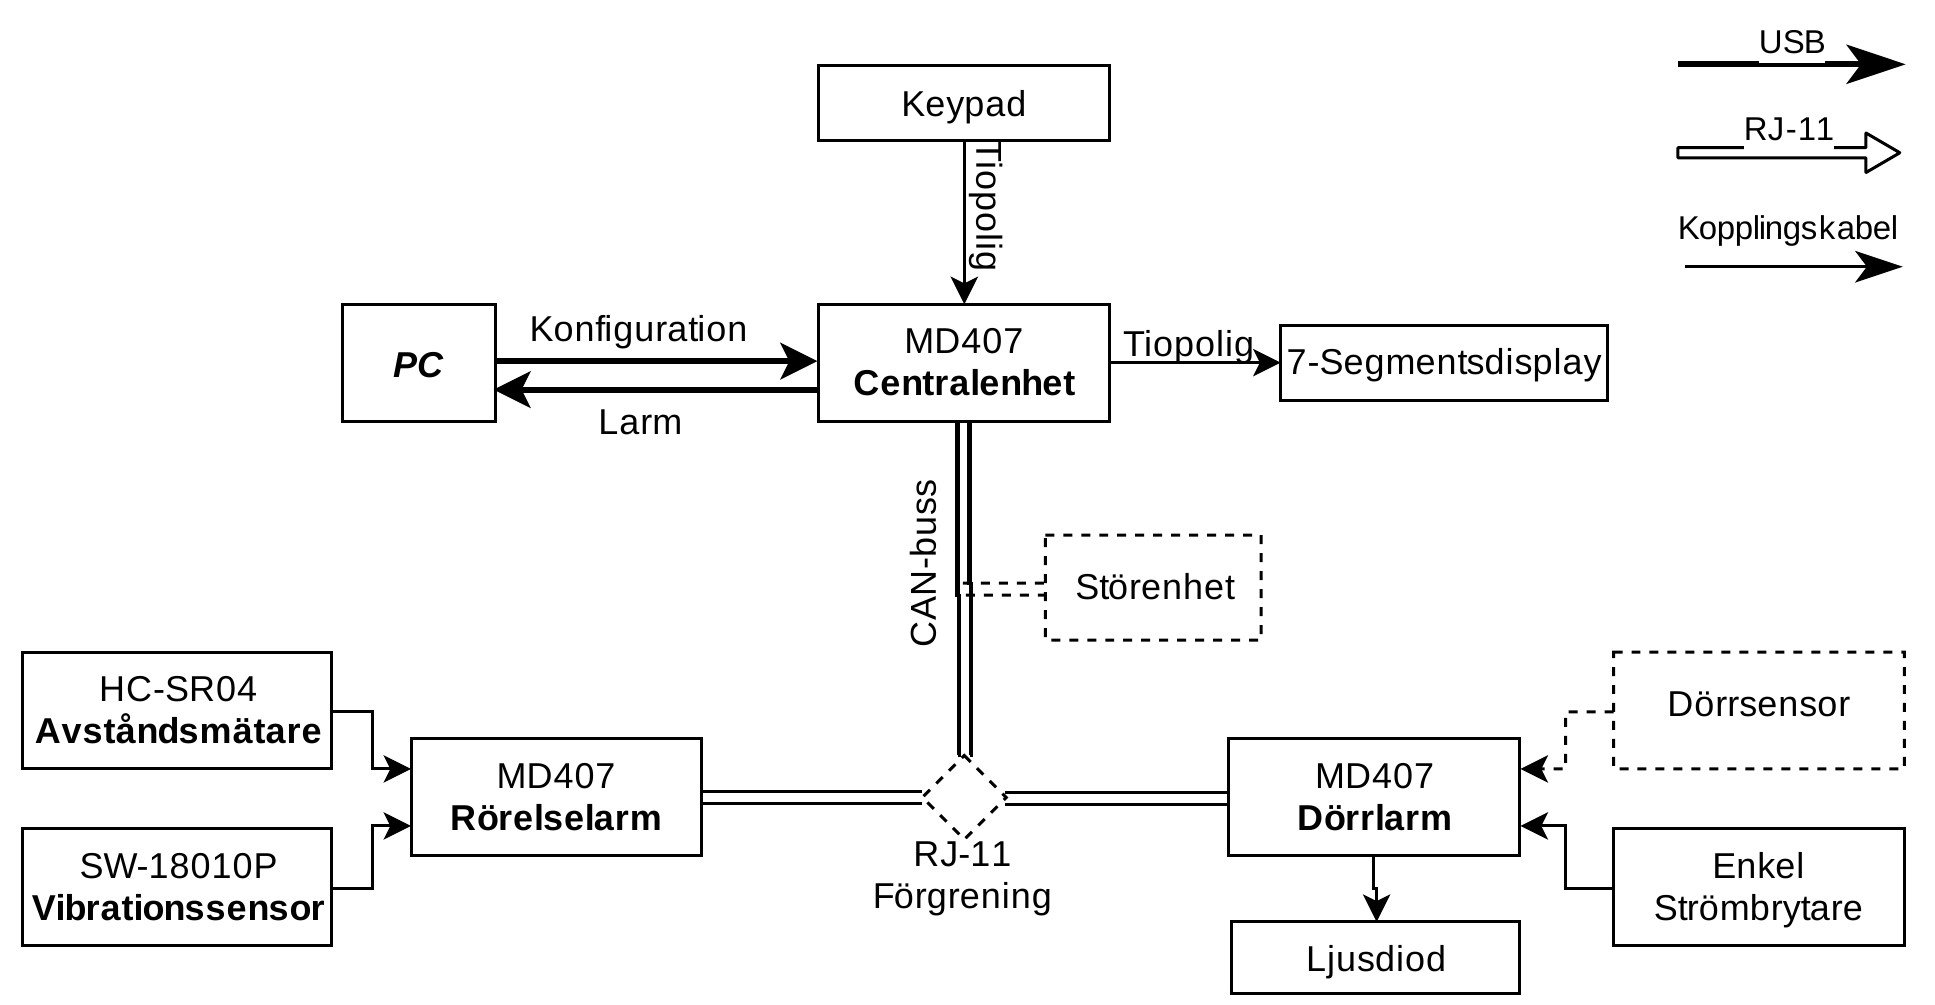
\includegraphics[width=1\textwidth]{figurer/HardvaraOversikt.jpg}
    \caption{Översikt Hårdvara}
    \label{fig:hårdvara}
\end{figure}

När centralenheten samt periferienheterna startar befinner de sig i konfigurationsläge, där de först konfigurerar sina egna enheter (USART, CAN-bussen, GPIO), varpå centralenheten skickar konfigurationer för sensorerna till periferienheterna, som de använder för att konfigurera sina respektive sensorer. Efter att ha konfigurerats går enehterna i var sin kontinuerlig loop. Periferienheterna mäter ständigt av sensorerna och skickar larm-meddelanden över CAN-bussen till centralenheten vid behov. Centralenheten skickar periodiskt konfigurationer till periferinheterna och larmar när de inte bekräftas.

En överblick av mjukvarans tidsflöde finns i Figur \ref{fig:tidsflöde}.

\begin{figure}[H]
    \centering
    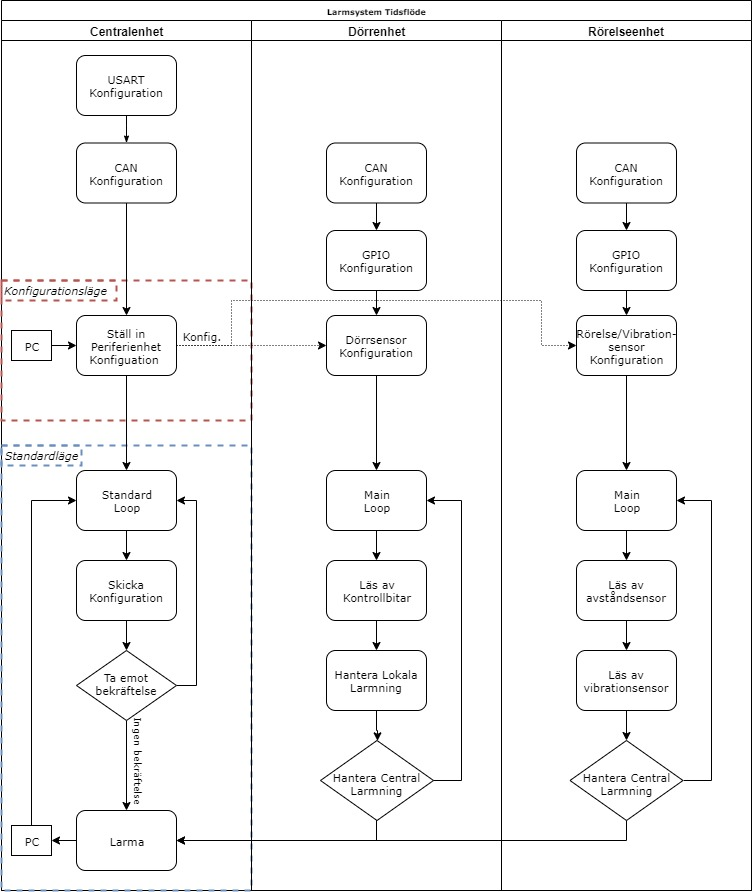
\includegraphics[width=1\textwidth]{figurer/TidsFlode.jpg}
    \caption{Tidsflöde Mjukvara}
    \label{fig:tidsflöde}
\end{figure}

\subsection{Delsystem }
\subsubsection{Centralenheten}
%\label{subsec:centralenhet}
Centralenheten styr och håller koll på övriga enheter.
 Inställningar görs via USART, varpå de vidarebefordras till rätt periferienhet via CAN (se \ref{can}).

Centralenheten har följande två lägen:

\begin{enumerate}
    \item Standardläge: Enheten väntar på larm-meddelanden från periferienheterna eller användarinput via USART. Dessutom skickar den regelbundet  konfigurationen för anslutna dörrar och sensorer till periferienheterna, som förväntas bekräfta konfigurationen. Om en enhet inte svarar efter ett förbestämt antal meddelanden går larmet.
    \item Konfigurationsläge: Enheten startar i detta läge.
     Här kan användaren konfigurera anslutna dörr- och
 rörelseenheter via USART. Användaren kan sätta centralenheten
      i detta läge via USART för att lägga till eller konfigurera periferienheter.
\end{enumerate}

För att kunna adressera olika periferienheter måste centralenheten tilldela dessa varsitt unikt id. Detta görs i konfigurationsläget genom att varje enhet som saknar id skickar en förfrågan via CAN. När centralenheten tar emot en sådan förfrågan från en periferienhet, skickar den tillbaka det lägsta lediga id:t och skapar en ny instans av en struktur som representerar periferienheten och lägger den i en
lista. Strukturen innehåller enhetens id och konfiguration (d.v.s. tider för varje dörr för dörrenheter respektive avstånd för varje avståndssensor och antal vibrationssensorer för rörelseenheter).
Id:t används för att addressera meddelanden till samt identifiera meddelanden från enheten. Det är också periferienhetens index i centralenhetens lista, vilket innebär att det är oerhört effektivt att hitta rätt enhet i listan när dess id har lästs i CAN-meddelandet.





\subsubsection{Dörrenheten}
%\label{subsec:Dörrenheten}

Dörrenheten är en av systemets fristående enheter och kräver ett MD407-kort. Ett kort kan stödja x dörrar.

Vid systemuppstart deteketeras alla stängda dörrar som är kopplade till MD407-kortet. En C-struktur kommer sedan initieras för varje dörr och fungera som en  datarepresentation för dörren. Denna datarepresentation är utrustad med följande värden:
\begin{itemize}
  \item {char id;}
  \item {int controlbits;}
  \item \textbf{char time\textunderscore{}Larm;}
  \item \textbf{char time\textunderscore{}Central\textunderscore{}Larm;}
  \item \textbf{int password;}
  \item int GPIO\textunderscore{}Lamp;
  \item int GPIO\textunderscore{}Read;
  \item int larmTick;
\end{itemize}

De fetstilta värdena är konfigurerbara för användaren, \textbf{time\textunderscore{}Larm} och \\ \textbf{time\textunderscore{}Central\textunderscore{}Larm} sätts med 10-sekunders intervall binärt med 8 bitar. Lösenordet \textbf{password} är 4 hexadecimala siffror som används för att låsa upp dörren på Keypaden.

Dörrenheten kan köras i lokaldrift men bör för bästa effekt köras uppkopplad mot centralenheten.\\
\subsubsection{Rörelseenheten}
Denna periferienhet använder avståndssensorer av modellen HC-SR04, och vibrationssensorer av modellen SW-18010P, som styrs av ett MD407-kort.
Vid uppstart av systemet skall alla inkopplade sensorer tilldelas ett id som säger vilken sorts sensor det är och numrerar dem.

\textbf{Avståndssensorn}: Aktiveras genom att MD407-kortet skickar en hög puls till sensorn i minst 10 mikrosekunder, 
 varpå sensorn skickar ut ultraljudsvågor och sänder en hög puls tills ultraljudsvågorna kommer tillbaks till MD407-kortet, där avståndet till närmaste föremål beräknas genom att mäta längden på pulsen. 
HC-SR04 kan mäta avstånd upp till 400cm och larmavståndet är justerbart från centralenheten.

\textbf{Vibrationssensorn}: Sensorn sänder ständigt en hög puls till MD407-kortet förutom när den känner av vibrationer, då den istället sänder en låg puls. 
Sensorns känslighet justeras fysiskt genom en komparator på sensorn.

\subsection{CAN-kommunikation}
\label{can}
Nedan finns dokumentationen av protokollet som tagits fram för
kommunikationen mellan enheterna. Därefter följer en beskrivning av hur kommunikationen har implementerats.
\subsubsection{Protokoll}
\section*{Grundidé}
\label{sec:grundide}

Centralenheten sparar all status och datainformation, denna information kopieras regelbundet till perferienheterna via konfigureringsmeddelanden. Centralenheten har 2 lägen.

\begin{enumerate}
	\item Standard running. Här lyssnar man på larm från periferienheterna. Dessutom skickar man regelbundet  konfigurationen för anslutna dörrar och sensorer. Periferienheten svarar ok, om den inte svarar efter ett antal meddelande larmar man.
	\item Vid uppstart är centralenheten i konfigurationsläge. Nu kan man via USART konfigurera anslutna dörrlarmsenheter samt lörelselarm.
\end{enumerate}

Varje perferienhet förväntas ha en unik fysisk adress som kommer användas vid tilldelning av ID adresser. Likt fysiska MAC adresser och logiska IP adresser i ethernet.

\section*{Bitfördelning i identifieringsdelen av meddelandet}
\label{sec:bitfördelning}

Totalt 11 bitar (Utan att utöka med 18 bitar till)
\begin{description}
	\item{0-2:} Första bitarna är meddelandetyp. 3 bitar dvs 8 meddelandetyper.
	\item{3:} en bit för riktning. Från/till centralenheten. Kan ses som en 4e bit i meddelandetypen.
	\item{4-10:} 7 bitar:
		Om riktning är till centralenheten är bitarna sändarens ID.
		Om riktningen är från centralenheten beskriver bitarna mottagarens ID.
		Innan enheten har en egen ID används bara ettor.
\end{description}


\section*{Meddelandetyper lista}
\label{sec:meddelandetyper}

\begin{table}[H]
	\begin{tabular}{|c|l|p{2.6cm}|p{6cm}|}
		\hline
		N& Riktning & Meddelandenamn & Beskrivning \\ \hline \hline
		0 & p -> c & Ack & Acknowledgement för senaste meddelandet. \\ \hline
		1 & p -> c & Skicka larm & Talar för centralenheten om någon dörr eller sensor larmar. \\ \hline
		3 & Båda & Skicka konfiguration & Skickar konfiguration till periferienheten kontinuerligt. Fungerar även som ping. Perferienheterna skickar sina konfigurationener i andra riktingen vid uppstart. Rörelselarmet har mätvärden i denna typ av meddelande. \\ \hline
		4 & c -> p & Tilldelning av ID & Centralenheten tilldelar en periferienhet dess ID. Enheten identifieras med dess fysiska adress i meddelandet. Detta meddelande skickas bara då centralenheten är i konfigurationsläge (läge  2). \\ \hline
		5 & p -> c & Ny enhet här & Centralenheten tilldelar en periferienhet dess ID. Enheten identifieras med dess fysiska adress i meddelandet. Detta meddelande skickas bara då centralenheten är i konfigurationsläge (läge  2). \\ \hline
	\end{tabular}
	\label{tab:meddelandetyper}
\end{table}

\section*{Detaljinformation angående meddelandetyperna}
\label{sec:detaljinfo}
\textbf{Skicka konfiguration} \\
I datadelen av meddelande för dörrlarm borde det finnas:
\begin{itemize}
	\item Ett par bitar för addressen till dörren i fråga.
	\item En aktiveringsbit per dörr.
	\item En bit per dörr för avaktivering av pågående larm.
	\item Ett par bitar för varje tidsfördröjning.
\end{itemize}

I datadelen av meddelande för rörelsesensorlarm borde det finnas:
\begin{itemize}
	\item En aktiveringsbit per sensor
	\item En bit per sensor för avaktivering av pågående larm.
	\item En bit per enhet för aktivering av automatisk översändning av “Skicka larm och mätvärden” meddelanden. Detta kommer användas vid konfiguration av avståndsgivare.
\end{itemize}

\section*{Todo}
\label{sec:todo}
Borde man ha olika meddelandetyper för “Skicka larm” beroende på vilken enhetstyp det rör sig om?

\subsubsection{Implementation}
För hantering av CAN-meddelanden har STM-biblioteket (se \ref{stm}) använts för inledande initiering, hantering av avbrott samt för att skicka meddelanden.
Utöver detta har det skapats ett system för hantering av mottagana meddelanden.
Detta har lösts med avbrott där hanteringsfunktionen paras ihop med filtret för tillhörande meddelande.
Hanteringsfunktionen anropas sedan av avbrottsrutinen då ett meddelande passerat filtret.
Denna lösning har valts då de flesta meddelanden naturligt hanteras med en kort hanteringsfunktion som inte kräver input från användaren.

Ett fall som är mer invecklat än en direkt hanteringsfunktion är vid konfiguration av avståndsgivare på rörelselarmet. I detta fall krävs input från användaren... \todo[inline]{Här borde de}\todo[inline]{Skriv färdigt föregående todo}




% Användarhandledning?

\section{Metoder}
\label{stm}
\subsection{Verifikation}
\todo[inline]{Har inte utfört några tester}
\subsection{Programbibliotek}
För att minska arbetet har programbiblioteket STM32\cite{stm}
använts. Detta har används vid initieringar av GPIO-portar, Systick med mera.

\section{Resultat och diskussion} % Kan dela upp dessa om vi vill.
% Detta avsnitt redovisar resultatet av genomförd verifirering av systemet; dels fördelarna, dels för komplett system. Detta avsnitt redovisar även resultatet av det slutgiltiga fysiska testet när hela systemet körs i skarpt läge. Ni ska främst redovisa resultat i form av funktionalitet, men ta ocks upp prestanda aspekter om dessa är viktiga. Diskutea hur väl ni lyckats med er slutprodukt i förhållande till er projektplan.
\todo[inline]{Vi har inget resultat än}
\section{Slutsats}
% Detta avsnitt innehåller en sammanfattning av konstruktionen och en diskussion av resultatet. Om detta är möjligt, dra slutsatser av ert projekt och identifiera förbättringsmöjligheter. (Vilka kan vara användbara för en beställare)
\todo[inline]{Vi har ingen slutsats än}

% Referenser enligtIEEE.
%För referenser
\bibliographystyle{IEEEtran}
\bibliography{referenser}

% Avslutningsvis så vill vi påminna om att projektets slutrapport, precis som projektplanen, ska vara projektintern, det väl säga att den ska beskriva det tekniska utvecklingsarbetet och bortse från att projektarbetet faktiskt organiserats inom ramen för en kurs.

\section{Bilagor}

\end{document}
